%  PowerDomains.tex
%  Document created by seblovett on seblovett-NETBOOK
%  Date created: Wed 19 Feb 2014 11:26:11 GMT
%  <+Last Edited: Mon 05 May 2014 11:59:12 BST by seblovett on seblovett-Ubuntu +>

\section{Power Techniques}
\subsection{Power Gating}



Leakage currents begin to occur in sub-micron technologies, typically lower than 100nm \cite{bsoul2010fpga, nair2009comparative}.
With each technology generation, gate leakage increases 30 fold \cite{bernstein2003design}.
Leakage currents can be classified as either sub-threshold currents or gate tunnelling. 
Sub-threshold currents occur when the voltage applied to the gate is lower than the transistor threshold voltage. 
The channel of the transistor during weak inversion still allows some current to flow from source to drain.
This current occurs when the transistor is off and is also exponentially dependant on $V_{th}$ \cite{borkar1999design}.
Gate tunnelling currents increase with thinner oxide layer \cite{m2002international}. 
A thin oxide results in electrons being able to pass through the gate into the substrate of the transistor. 
%This thin gate results in electrons passing through it, into the circuit causing leakage. 
Gate tunnelling occurs when the transistor is active \cite{nair2009comparative}.
Figure \ref{fig:leakage} shows where these leakage currents occur on an NMOS transistor.

\begin{figure}
\centering
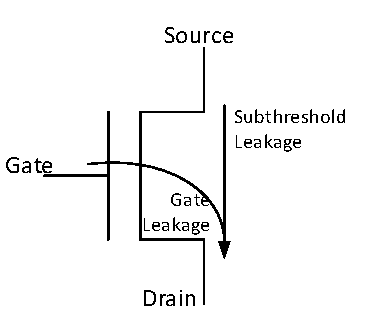
\includegraphics[width=0.3\textwidth]{Figures/leakage.pdf}
\caption{The locations of gate and subthreshold leakage on an NMOS transistor}
\label{fig:leakage}
\end{figure}
%\todo[inline]{\cite{altera2005} has a good figure of the leakage currents}



\subsubsection{Theory}

Power gating, in principle, is where the power to a module is switched off when not in use. 
By doing this, the module does not consume any power. 
It can be achieved by using either a header or a footer switch to disable either the supply connection or the ground connection respectively. 
Figure \ref{fig:powerswitches} shows the realisation of the power gating circuits.

\begin{figure}[h]
\centering
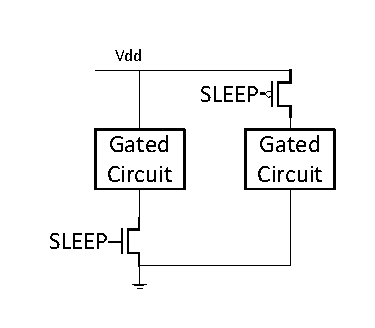
\includegraphics[width=0.3\textwidth]{Figures/powergating_switches.pdf}
%\subfigure[Header PMOS transistor]{Figures/powergating_switches_header.pdf}
%\subfigure[Footer NMOS transistor]{Figures/powergating_switches_footer.pdf}
\caption{Circuit diagram showing the use of power gating transistors.}%footer switches (left) or header switches (right).}
\todo[inline]{Break this into two subfigures}
\label{fig:powerswitches}
\end{figure}

%\begin{figure}[t!]
%    \centering
%    \begin{subfigure}{0.5\textwidth}
%        \centering
%        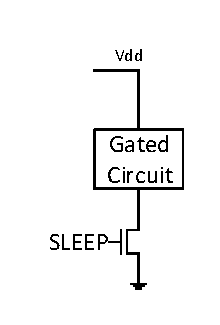
\includegraphics{Figures/powergating_switches_header.pdf}
%        \caption{Header PMOS transistor}
%    \end{subfigure}%
%    ~ 
%    \begin{subfigure}{0.5\textwidth}
%        \centering
%        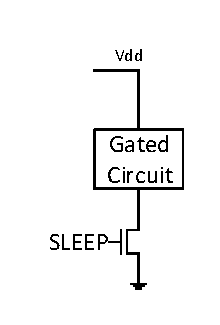
\includegraphics{Figures/powergating_switches_footer.pdf}
%        \caption{Footer NMOS transistor}
%    \end{subfigure}
%\caption{Circuit diagrams showing the use of power gating transistors.}%footer switches (left) or header switches (right).}
%\label{fig:powerswitches}
%\end{figure}


Although the theory of operation is simple, the technique poses many issues in the implementation.
Firstly, as the module is floating, the outputs are undefined.
This can cause the gates in another module to short circuit - at an input voltage of $ V_{dd} / 2 $, both the NMOS and PMOS transistors will be on, resulting in a direct line from supply to ground. 
The solution to this is is to add logic gates with a `clamp' signal. 
This could be either an \texttt{AND} gate, of which the clamp signal is active low, or an \texttt{OR} gate with an active high clamp. 
This added logic is needed per output signal of the power gated module.

The second issue that power gating raises is when the gated module contains sequential logic. 
By removing the power to the sequential logic, the state is lost. 
This can then cause issues as state retention may be necessary, as well as low power.
The solution is to use a state retention register. 
There is a timing overhead involved to store the register before putting the device to sleep, disabling the majority of the circuit. 
State retention registers also require an ungated power supply, meaning all power gated modules require two supplies; one which is gated and one constant supply.

The final aspect of power gating that needs addressing is the power management.
The power manager is responsible for when to gate the module. % on and off.
As well as the control of the sleep transistors, the power manager is also responsible for the stopping the clock, clamping the outputs and saving the state to the state retention mechanism.

There is a large overhead in the additional circuitry needed for power gating. 
The main increase is due the state retention registers as these can require 20\% more area in silicon \cite{stateretarea}. 
Other techniques exist to avoid this, such as the use of the scan path to quickly clock the state in and out to/from memory.
Digital signal processing, however, would not need this as it is data dependent. 
Processors with cache have a large amount of state data, so state retention registers are needed here.

When footer switches are used, the voltage that at the source of the NMOS is known as the virtual ground (VGND). When the footer is active, VGND $\approx$ GND. When off, VGND $\approx V_{dd}$.
A full realisation of a power gated circuit is shown in figure \ref{fig:powergated}. 


\begin{figure}
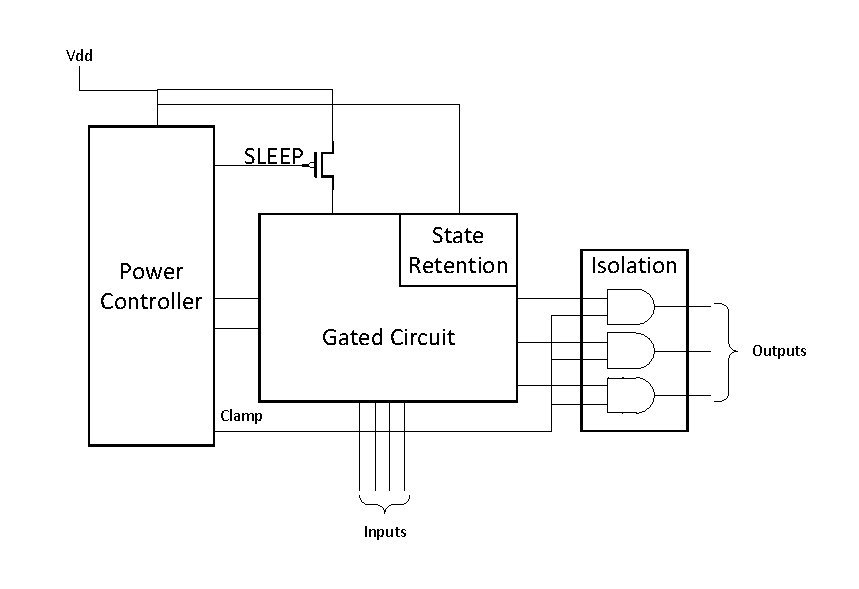
\includegraphics[width=0.5\textwidth]{Figures/powergating_full.pdf}
\caption{The realisation of a power gated module. State retention, isolation and a power manager are all needed}
\label{fig:powergated}
\end{figure}


\subsubsection{Synthesis Techniques}

%Fine and coarse grain techniques
Power gating can be split into two techniques, fine and coarse grain.
Fine grain gating is where individual cells (e.g. in ASIC) have their own gating transistor. 
Coarse grain techniques are where gating transistors are applied on a larger module scale.
\cite{nair2009comparative} compares the fine grain and coarse grain methods on a 65nm FPGA technology. 
Here, a SRAM block is used as the test circuit. 
Fine grain, in this case, is where the memory of each cell is individually gated, and coarse grain is where a $16 \times 1$ SRAM module is gated. 
It was conclusively shown that coarse grain gating reduced power consumption more than fine grain due to being able to turn off the read/write circuitry. 


%Multi sleep mode
When deciding to sleep a module, there are a number of overheads.
Due to the charging / discharging of the gated circuit (depending on the use of header or footer switches), when the circuit is re-enabled there is an amount of time needed to allow the capacitors to return to normal \cite{abdollahi2005effective}.
This is referred to as the wake-up time and can also include the time to restore state, if applicable.
The (dis)charging can also pose ground bounce issues to the device due to the sudden draw of current \cite{kim2003understanding,chang1997analysis}. 

This wake up time can then impact the performance of the device - if more energy is consumed waiting for the disabled module than it would have consumed being awake, the overall power is not reduced.
\cite{kim2004experimental} discusses a method where an intermediate power saving mode is introduced.
This is done by using a standard footer power gating NMOS. 
An extra PMOS is then added in parallel with the power gating switch. 
Table \ref{tab:kim} summarises the states of the transistors in the circuit in figure \ref{fig:kim}

The RUN and COLD states operate as previously discussed. 
The PARK state, however, is where the virtual ground voltage does not rise to $V_{dd}$ due to the PMOS conducting. 
The virtual ground is at the threshold voltage of the PMOS, so the leakage current is less than in the RUN state but not so high that state retention is needed. 
This drastically reduces the wake up overhead of the circuit. 
\todo[inline]{consistency of wake up / wake-up}
\todo[inline]{- replaced by : in some places too}
\begin{figure}
\centering
%\missingfigure{\cite{kim2004experimental} power states circuit}
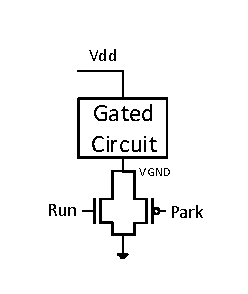
\includegraphics[width=0.3\textwidth]{Figures/powergating_kim.pdf}
\caption{Middle power state implementation used in \cite{kim2004experimental}}
\label{fig:kim}
\end{figure}

\begin{table}
\caption{Power saving modes of \cite{kim2004experimental}}
\label{tab:kim}
\centering
\begin{tabular}{|c|c|c|c|}\hline
State Name & NMOS State & PMOS State & Virtual Ground Voltage (V)\\ \hline
RUN  & ON   & OFF  & GND \\
COLD & OFF  & OFF  & $V_{DD}$ \\
PARK & OFF  & ON   & $V_{th}$ PMOS \\ \hline
\end{tabular}
\end{table}

A further improvement to this single extra state is proposed in \cite{singh2007enhanced}. 
Here, multiple intermediate power states are implemented by using different sub-threshold gate voltages on the NMOS footer switch. 
The compromise of wake up time against leakage reduction can then be more finely controlled to best suit the circuit.
In general, the closer the virtual ground is to ground, the more leakage current occurs, but a faster wake up is available. 

Sub Clock Power Gating employs the same basic idea, but in a different manner \cite{mistry2011sub}.
This technique reduces the leakage power of a circuit during the active state of the module.
It utilises the fact that the combinational logic is not used for half of the clock cycle in synchronous circuits.
The combinational logic blocks can then be gated for half of the clock cycle.
The result is that the combinational logic is turned off regularly. 
The timings of the signals are seen in figure~\ref{fig:scpg:timing}.

\begin{figure}
%\missingfigure{The power gating timing from \cite{mistry2011sub}.}
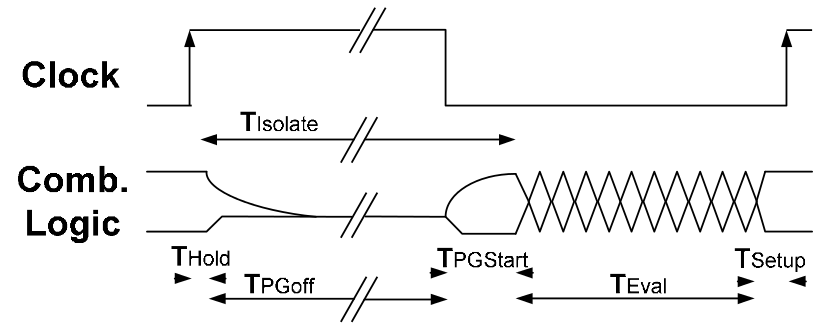
\includegraphics[width=0.4\textwidth]{Figures/scpg_timings.png}
\caption{The signal timings for Sub Clock Power Gating. Reproduced from \cite{mistry2011sub}}
\label{fig:scpg:timing}
\end{figure}

\todo[inline]{Figure / figure}

As this method only affects the combinational blocks, the sequential registers are not gated.
This results in no need for state retention registers.
Also, due to the reliance on the clock for the gating, the power management module is reduced to a combinational function depending on the clock. 
This logic can be seen in figure~\ref{fig:scpg:gate}. 
The isolation circuit also needs to be dependent on the clock.
This is seen in Figure~\ref{fig:scpg:iso}.
This circuit is needed to isolate during the high period of the clock. 
It also must assert the isolate signal until the combinational logic block is recharged. 
The isolation signal must be high when Virtual $V_{dd}$ is low and the clock is low, or when the clock is high. 

\todo[inline]{Could be better to have the isolation / gating circuit instead of the clock gating with AND gate.}
\begin{figure}
%\missingfigure{The power gating circuit from \cite{mistry2011sub}.}
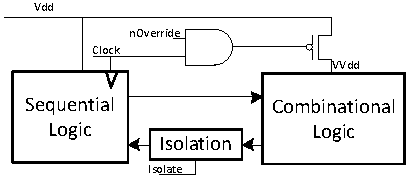
\includegraphics[width=0.4\textwidth]{Figures/mistry_gating.pdf}%scpg_circuit.png}
\caption{The power management circuitry needed to implement Sub Clock Power Gating. Reproduced from \cite{mistry2011sub}}
\todo[inline]{redo this. Add isolation circuit too}
\label{fig:scpg:gate}
\end{figure}
\begin{figure}
%\missingfigure{The power gating circuit from \cite{mistry2011sub}.}
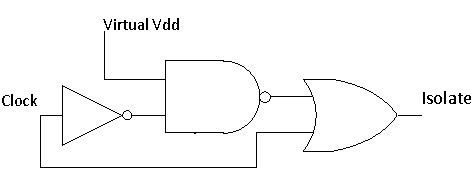
\includegraphics[width=0.4\textwidth]{Figures/mistry_isolation.pdf}%scpg_circuit.png}
\caption{The isolation managing circuit. Reproduced from \cite{mistry2011sub}}
\label{fig:scpg:iso}
\end{figure}

It was found that Sub Clock Power Gating increased the energy efficiency of a multiplier and microprocessor by 45$\times$ and 2.5$\times$ respectively \cite{mistry2011sub}.
This method overcomes the main additions needed (state retention and power manager) to implement power gating, with only isolation and the gating transistors needed. 

%\subsection{Power Scaling}
%
%\inote{I want to try and find use of two modules, one with a Low $V_t$ for high performance, high power, and a high $V_t$ for low performance, low power, which can be switched between. 
%If not, just look at multi $V_t$ technologies}
%%\inote{What actually am I wanting to discuss here?}
%\inote{Or I could look into adaptive body bias?}
%
%\subsubsection{Theory}
%
%
%\subsubsection{Synthesis Techniques}
%
%
%\subsection{Power Domains}
%
%\subsubsection{Theory}
%
%\subsubsection{Synthesis}
